\question[30] Elige la respuesta para cada pregunta, a partir de las imágenes de la figura \ref{fig:cerditos}.

\begin{multicols}{2}
\begin{parts}

\begin{minipage}[t][][t]{0.35\textwidth}\begin{figure}[H]
\begin{center}
\centering
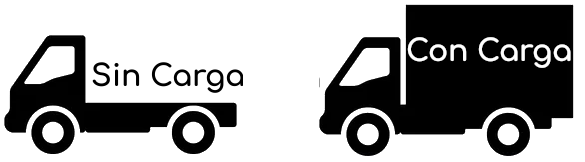
\includegraphics[width=0.5\linewidth]{camionesdecarga01}
\captionof{figure}{Representación de dos vehículos de carga.}
\label{fig:cerditos}
\end{figure}

\part ¿Cuál de ellos será más fácil poner en movimiento?

\begin{choices}
    \choice El camión sin carga.
    \choice El camión cargado.
    \choice Los dos camiones requieren el mismo esfuerzo.
\end{choices}


\part ¿Cuál podría aumentar más rápido su velocidad?
\begin{choices}
    \choice El camión sin carga.
    \choice El camión cargado.
    \choice Los dos camiones aumentan su velocidad con la misma rapidez.
\end{choices}


\part Si ambos camiones se movieran a la misma velocidad,
¿a cuál de ellos le resultaría más fácil frenar?

\begin{choices}
    \choice El camión sin carga.
    \choice El camión cargado.
    \choice Los dos camiones requieren el mismo esfuerzo.
\end{choices}

\part  ¿Cuál de los camiones podría tomar una curva con más
facilidad si ambos se están moviendo a la misma velocidad?

\begin{choices}
    \choice El camión sin carga.
    \choice El camión cargado.
    \choice Los dos camiones requieren el mismo esfuerzo.
\end{choices}

%\vspace{1cm}

\part Si el camión cargado va dejando gradualmente parte de su cargamento mientras el
conductor pisa el acelerador con la misma fuerza y mantiene el camión en la misma dirección,
¿qué pasa con su rapidez?

\begin{choices}
    \choice La rapidez del cami\'on aumenta.
    \choice La rapidez del cami\'on disminuye.
    \choice La rapidez del cami\'on no cambia.
\end{choices}
%   \end{multicols}
% \end{parts}

% \newpage

% \question Elige la respuesta para cada pregunta, a partir de las imágenes de la figura \ref{fig:camiones2}.\\

% \begin{parts}
%     \begin{minipage}[t]{0.25\linewidth}
%         
\begin{minipage}[t][][t]{0.35\textwidth}\begin{figure}[H]
\begin{center}
%             \centering
%             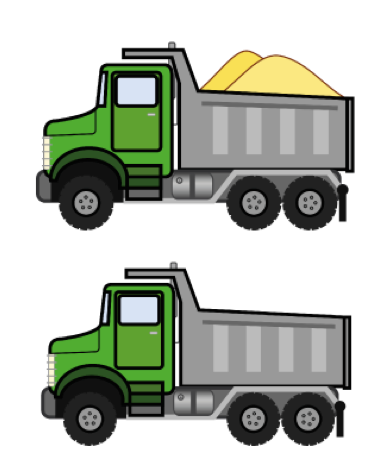
\includegraphics[width=\linewidth]{camiones2.png}
%             \captionof{figure}{}
%             \label{fig:camiones2}
%         \end{figure}
%     \end{minipage}\hfill
%     \begin{minipage}[t]{0.7\linewidth}
%        \part ¿Cuál de ellos será más difícil poner en movimiento?
%         \begin{choices}
%             \choice El camión sin carga.
%             \choice Los dos camiones requieren el mismo esfuerzo.
%             \choice El camión cargado.
%         \end{choices}

%        \part ¿Cuál podría aumentar más lento su velocidad?

%         \begin{choices}
%             \choice El camión sin carga.
%             \choice Los dos camiones aumentan su velocidad con la misma rapidez.
%             \choice El camión cargado.
%         \end{choices}

%        \part Si ambos camiones se movieran a la misma velocidad,
%         ¿a cuál de ellos le resultaría más difícil frenar?

%         \begin{choices}
%             \choice El camión sin carga.
%             \choice Los dos camiones requieren el mismo esfuerzo.
%             \choice El camión cargado.
%         \end{choices}
%     \end{minipage}

%    \part  ¿Cuál de los camiones podría tomar una curva con más
%     dificultad si ambos se están moviendo a la misma velocidad?

%     \begin{choices}
%         \choice El camión sin carga.
%         \choice Los dos camiones requieren el mismo esfuerzo.
%         \choice El camión cargado.
%     \end{choices}

%    \part Si se reduce la carga de arena de tal manera que la masa
%     del camión sea la mitad de su masa inicial, mientras el conductor pisa el
%     acelerador con la misma fuerza y mantiene el camión en la misma dirección,
%     ¿qué pasa con la acelaración del camión?

%     \begin{choices}
%         \choice Aumenta al doble.
%         \choice Disminuye a la mitad.
%         \choice No cambia.
%     \end{choices}

% \end{parts}

% \newpage
% \question Elige la respuesta para cada pregunta, a partir de las imágenes de la figura \ref{fig:camiones3}.


\part ¿Cuál podría aumentar más rápido su velocidad?

\begin{choices}
    \choice El autobús con más niños.
    \choice El autobús con menos niños.
    \choice Los dos autobuses aumentan su velocidad con la misma rapidez.
\end{choices}

\part Si ambos autobuses se mueven a la misma velocidad, ¿a cuál de ellos le resultaría más difícil frenar?

\begin{choices}
    \choice Los dos autobuses requieren el mismo esfuerzo.
    \choice  El autobús con menos niños.
    \choice El autobús con más niños.
\end{choices}

\part  Si la masa del segundo autobús es la mitad del primero
y ambos conductores pisan el acelerador con la misma fuerza y mantienen el autobús en la misma dirección, ¿qué pasa con su aceleración?

\begin{choices}
    \choice Se mantiene igual.
    \choice Es el doble que la del primero.
    \choice Es la mitad de la del primero.
\end{choices}

\part  Si el conductor del autobús baja a algunos niños,
de tal manera que su masa sea sólo un cuarto de su masa inicial, cuando el conductor pisa el acelerador con la misma fuerza y mantiene el camión en la misma dirección, ¿qué pasa con su acelaración?

\begin{choices}
    \choice Aumenta cuatro veces.
    \choice Se mantiene igual.
    \choice Disminuye a la cuarta parte.
\end{choices}

\part El conductor del autobús da vuelta hacia la derecha y los niños
sienten una \emph{fuerza} que los empuja. ¿En qué dirección sienten los niños esta fuerza?

\begin{choices}
    \choice Los niños sienten que son empujados hacia abajo.
    \choice Los niños sienten que son empujados hacia la derecha del autobús.
    \choice Los niños sienten que son empujados hacia la izquierda del autobús.
\end{choices}
\end{parts}
\end{multicols}
